\documentclass[a4paper, 11pt]{article}
\usepackage{slashbox}
\usepackage{pgfplots}
\pgfplotsset{/pgf/number format/use comma,compat=newest}

\begin{document}
\section*{Insertion sort vs quick sort}
\vspace{0,4 cm}
L'obiettivo di questo esercizio consiste nel valutare le prestazione degli algoritmi di ordinamento insertion sort e quick sort. Per entrambi gli algoritmi si valuta la prestazione su array non ordinati e nel caso peggiore (array in ordine decrescente per insertion sort e in ordine crescente per quick sort). Inoltre per insertion sort si valuta il funzionamento anche nel caso migliore, cioè quando l'array inserito è in ordine crescente.

\vspace{0,5 cm}
Insertion sort è un algoritmo di ordinamento iterativo, efficace se applicato a pochi elementi. L'insieme di elementi considerato ad ogni iterazione risulta ordinato, poiché per ognuna di esse l'algoritmo inserisce,nella corretta posizione, un elemento all'interno di un sottoarray già ordinato. Il tempo di esecuzione dipende da quanto gli elementi dell'array originario sono ordinati e da quante posizioni un elemento deve visitare  per essere inserito. Il tempo di esecuzione per un array di $n$ elementi è compreso fra $n$ (caso migliore) e $n^{2}$ (caso peggiore).

\vspace{0,5 cm}
Quick sort è un algoritmo di ordinamento ricorsivo \textit{divide et impera}.\\
Un algoritmo \textit{divide et impera}, divide l'array in due sottoarray per poi chiamarsi nuovamente su entrambi. In quick sort, il punto in cui dividere l'array è dato dalla funzione \emph{partition}. Questa operazione si ripete finché gli array risultano composti da un solo elemento, per essere poi combinati. Il tempo di esecuzione dipende da quanto sono bilanciati i sottoarray, cioè da quanta differenza esiste fra le lunghezze dei due sottoarray in cui un array è diviso. Il tempo di esecuzione oscilla fra $n\log_2{n}$ (caso migliore, cioè con sottoarray sempre bilanciati) e $n^2$ (caso peggiore).

\vspace{0,5 cm}
Gli algoritmi sono stati implementati in Python e tutti i test di performance sono stati svolti con \emph{unittest}. Nel file dedicato ad \emph{unittest},  ogni esecuzione del \emph{main} genera 15 array:
\begin{itemize}
\item 5 array con ordinamento casuale (10, 100, 1000, 10000, 100000 elementi) che risultano diversi ad ogni esecuzione
\item 5 array ordinati con ordine crescente (10, 100, 1000, 10000, 100000 elementi)
\item 5 array ordinati con ordine decrescente (10, 100, 1000, 10000, 100000 elementi)
\end{itemize}
attraverso la funzione \emph{setUp()}.
	
\vspace{0,5 cm}
L'obiettivo dei test è controllare l'effettivo funzionamento di questi due algoritmi e il loro tempo di esecuzione.\\
Dai test svolti sugli array sopra descritti, ci si aspetta che l'algoritmo quick sort sia più veloce di insertion sort al crescere del numero $n$ di elementi. Per entrambi gli algoritmi di ordinamento è stato fissato un tempo di esecuzione massimo di 2 minuti, oltre il quale l'esecuzione viene interrotta. I test eseguiti sono stati 10 volte.

\vspace{0,5 cm}
Per insertion sort sono stati ottenuti i seguenti risultati:
\begin{center}
\footnotesize
\setlength{\tabcolsep}{5 pt}
\hspace*{-4,1 cm}
\begin{tabular}{c | c c c c c | c c c c c | c c c c c |}
\cline{2-16}
& \multicolumn{5}{| c |}{Random} & \multicolumn{5}{| c |}{Caso peggiore} & \multicolumn{5}{| c |}{Caso migliore} \\
\hline
\multicolumn{1}{| c |}{\backslashbox{Prova }{ N° dati}} & 10 & 100 & 1000 & 10000 & 100000 & 10 & 100 & 1000 & 10000 & 100000 & 10 & 100 & 1000 & 10000 & 100000\\
\hline
\multicolumn{1}{| c |}{1} & 0 & 0 & 0,17184 & 16,84326 & $>$120 & 0 & 0 & 0,18744 & 19,34493 & $>$120 & 0 & 0 & 0 & 0,01562 & 0,0625\\
\hline
\multicolumn{1}{| c |}{2} & 0 & 0 & 0,15617 & 16,46961 & $>$120 & 0 & 0 & 0,18746 & 19,12216 & $>$120 & 0 & 0 & 0 & 0,01562 & 0,06249\\
\hline
\multicolumn{1}{| c |}{3} & 0 & 0 & 0,18186 & 16,68695 & $>$120 & 0 & 0 & 0,18998 & 19,15717 & $>$120 & 0 & 0 & 0 & 0 & 0,04686\\
\hline
\multicolumn{1}{| c |}{4} & 0 & 0 & 0,18746 & 16,45171 & $>$120 & 0 & 0 & 0,20308 & 18,82525 & $>$120 & 0 & 0 & 0 & 0 & 0,04687\\
\hline
\multicolumn{1}{| c |}{5} & 0 & 0 & 0,17184 & 16,84345 & $>$120 & 0 & 0 & 0,17318 & 19,09465 & $>$120 & 0 & 0 & 0 & 0 & 0,06249\\
\hline
\multicolumn{1}{| c |}{6} & 0 & 0 & 0,17184 & 17,04365 & $>$120 & 0 & 0 & 0,17183 & 19,51302 & $>$120 & 0 & 0 & 0 & 0 & 0,04691\\
\hline
\multicolumn{1}{| c |}{7} & 0 & 0 & 0,20308 & 17,27844 & $>$120 & 0 & 0 & 0,20313 & 20,40876 & $>$120 & 0 & 0 & 0 & 0,01562 & 0,06251\\
\hline
\multicolumn{1}{| c |}{8} & 0 & 0 & 0,15622 & 16,89078 & $>$120 & 0 & 0,01562 & 0,17183 & 19,1869 & $>$120 & 0 & 0 & 0 & 0,01562 & 0,06248\\
\hline
\multicolumn{1}{| c |}{9} & 0 & 0 & 0,17185 & 16,98244 & $>$120 & 0 & 0 & 0,17183 & 18,60975 & $>$120 & 0 & 0 & 0 & 0 & 0,04687\\
\hline
\multicolumn{1}{| c |}{10} & 0 & 0 & 0,16642 & 17,45238 & $>$120 & 0 & 0 & 0,18746 & 19,81163 & $>$120 & 0 & 0 & 0 & 0 & 0,04686\\
\hline
\end{tabular}
\begin{figure}[h]
\centering
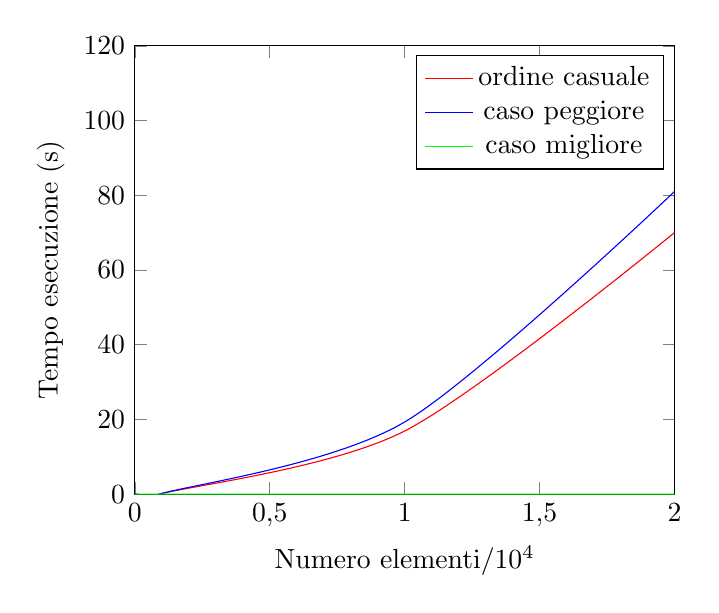
\begin{tikzpicture}
\begin{axis}[xmin=0, xmax=2, ymin=0,ymax=120, xlabel=Numero elementi$/10^4$, ylabel=Tempo esecuzione (s)]
\addplot[smooth, red]
coordinates{(0,0) (0.001,0) (0.01,0) (0.1,0.17386) (1,16.89427) (2,70)};
\addplot[smooth, blue]
coordinates{(0,0) (0.001,0) (0.01,0.00156) (0.1,0.18472) (1,19.30742) (2,81)};
\addplot[smooth, green]
coordinates{(0,0) (0.001,0) (0.01,0) (0.1,0) (1,0.00625) (2,0.01562)};
\legend{ordine casuale,caso peggiore,caso migliore}
\end{axis}
\end{tikzpicture}
\end{figure}
\end{center}

\vspace{-0,5 cm}
I risultati riportati sono espressi in secondi sia per la tabella che per diagramma cartesiano. Per il diagramma, come si può notare, è stato scelto di interrompere la rappresentazione a 20000 elementi, questo perché l'inserimento di dati fino a 100000 elementi non avrebbe permesso di apprezzare bene la differenza fra i vari tipi di array inseriti. In compenso, osservando i dati della tabella e la crescita delle funzioni, si può capire che, ad eccezione del caso migliore, gli array con 100000 elementi necessitano di più di 120 secondi per essere ordinati.
\newpage
Per quick sort abbiamo invece ottenuto i seguenti risultati:

\vspace{0,7 cm}
\begin{center}
\footnotesize
\setlength{\tabcolsep}{5 pt}
\begin{tabular}{c | c c c c c | c c c |}
\cline{2-9}
& \multicolumn{5}{| c |}{Random} & \multicolumn{3}{| c |}{Caso peggiore}\\
\hline
\multicolumn{1}{| c |}{\backslashbox{Prova }{ N° dati}} & 10 & 100 & 1000 & 10000 & 100000 & 10 & 100 & 1000\\
\hline
\multicolumn{1}{| c |}{1} & 0 & 0 & 0,01562 & 0,18746 & 7,83413 & 0 & 0,01561 & 0,29681\\
\hline
\multicolumn{1}{| c |}{2} & 0 & 0 & 0,01562 & 0,18746 & 7,85057 & 0 & 0,01561 & 0,28119\\
\hline
\multicolumn{1}{| c |}{3} & 0 & 0 & 0,01562 & 0,20547 & 7,80365 & 0 & 0 & 0,31255\\
\hline
\multicolumn{1}{| c |}{4} & 0 & 0 & 0,01563 & 0,18745 & 7,75573 & 0 & 0 & 0,29687\\
\hline
\multicolumn{1}{| c |}{5} & 0 & 0 & 0,01562 & 0,18745 & 7,6658 & 0 & 0 & 0,29681\\
\hline
\multicolumn{1}{| c |}{6} & 0 & 0 & 0,01561 & 0,18747 & 7,88184 & 0 & 0 & 0,31243\\
\hline
\multicolumn{1}{| c |}{7} & 0 & 0 & 0,01562 & 0,20308 & 7,96078 & 0 & 0,01562 & 0,31265\\
\hline
\multicolumn{1}{| c |}{8} & 0 & 0 & 0,01562 & 0,18746 & 7,64869 & 0 & 0 & 0,29681\\
\hline
\multicolumn{1}{| c |}{9} & 0 & 0 & 0,01562 & 0,20308 & 7,61693 & 0 & 0,00379 & 0,29426\\
\hline
\multicolumn{1}{| c |}{10} & 0 & 0 & 0,01562 & 0,18746 & 7,67918 & 0 & 0 & 0,28119\\
\hline
\end{tabular}
\vspace{1 cm}
\begin{figure} [h]
\centering
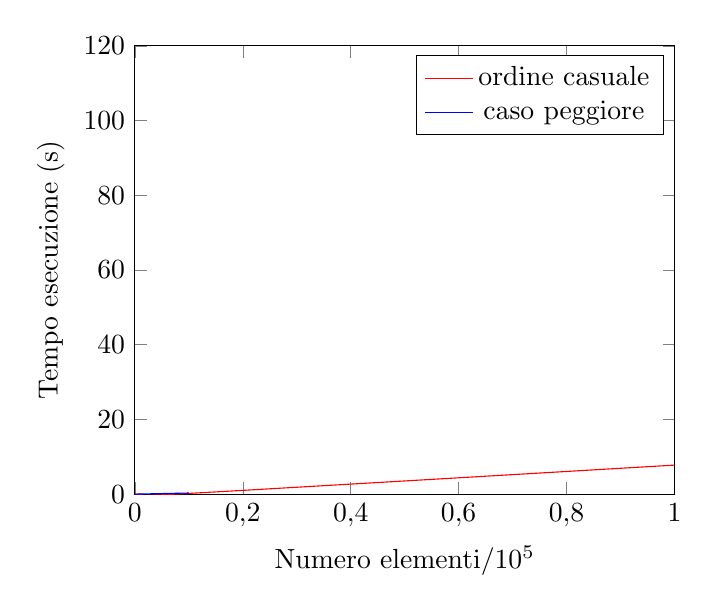
\begin{tikzpicture}
\begin{axis}[xmin=0, xmax=1, ymin=0,ymax=120, xlabel=Numero elementi$/10^5$, ylabel=Tempo esecuzione (s)]
\addplot[smooth, red]
coordinates{(0,0) (0.0001,0) (0.001,0) (0.01,0.01562) (0.1,0.19238) (1,7.76973)};
\addplot[smooth, blue]
coordinates{(0,0) (0.0001,0) (0.001,0.00506) (0.1,0.29816)};
\legend{ordine casuale,caso peggiore}
\end{axis}
\end{tikzpicture}
\end{figure}
\end{center}
\vspace{0,5 cm}

Come si può notare, l'algoritmo di quick sort è più veloce rispetto a quello di insertion sort, per il quale, causa tempi di esecuzione troppo piccoli, non abbiamo neanché potuto apprezzare la sua efficacia su un ristretto numero di elementi.\\
Nei dati sopra riportati, si noti inoltre la mancanza di prove effettuate sul quick sort nel caso peggiore per 10000 e 100000 elementi. Ciò è dovuto al fatto che l'ambiente di sviluppo rileva un errore di \emph{stack overflow} per funzioni che superano le 1000 ricorsioni.
\newpage
\textbf{Documentazione codice}

\vspace{0,7 cm}
Il codice, implementato con Python sull'ambiente di sviluppo PyCharm, è stato diviso su due file:
\begin{itemize}
\item esercizio\textunderscore{1}, nel quale la classe \emph{Array} permette di istanziare array di dimensione $n$ con ordine casuale, crescente o decrescente. La classe ha come metodi interni i due algoritmi di ordinamento, cosicché quest'ultimi siano eseguibili direttamente dall'oggetto istanziato. In ingresso, il costruttore richiede l'inserimento della lunghezza \emph{n} e del tipo di array (inserire 0 per avere elementi non ordinati, 1 con ordine crescente e 2 con ordine decrescente);
\item test\textunderscore{esercizio1}, nel quale, i test, scritti in \emph{unittest}, sono implementati in una classe \emph{TestArray}. Per ogni esecuzione di un algoritmo di ordinamento, viene controllato che l'array risultante sia ordinato entro il tempo limite. All'interno della classe sono presenti due metodi per i test e la funzione \emph{setUp()}. I test relativi a insertion sort sono svolti nel metodo \emph{test\textunderscore{insertion\textunderscore{sort()}}}, mentre quelli relativi a quick sort sono in \emph{test\textunderscore{quick\textunderscore{sort()}}}
\end{itemize}

\vspace{0,4 cm}
Per ogni esecuzione del file di test, gli array generati sono 15.\\
I 5 non ordinati sono gli stessi per entrambi gli algoritmi di ordinamento, mentre i 5 per il caso migliore di insertion sort sono gli stessi usati per il caso peggiore quick sort (array con ordine crescente). I 5 rimanenti sono quelli usati per il caso peggiore di insertion sort (array con ordine decrescente).
\end{document}
